\documentclass[a4paper,ngerman,12pt]{scrartcl}

\usepackage[utf8]{inputenc}
%\usepackage[ansinew]{inputenc}

\usepackage[ngerman]{babel}

\usepackage{amsmath,amsthm,amssymb,stmaryrd,color,graphicx}
\usepackage{setspace}
\usepackage{bussproofs}
\usepackage{array}
\usepackage{comment}

\usepackage{enumitem}

\usepackage{units}

\usepackage[protrusion=true,expansion=true]{microtype}

\usepackage{lmodern}

\usepackage{hyperref}
\usepackage{cleveref}
\usepackage{wrapfig}

\newcommand{\RR}{\mathbb{R}}
\newcommand{\CC}{\mathbb{C}}
\newcommand{\ZZ}{\mathbb{Z}}
\newcommand{\NN}{\mathbb{N}}
\newcommand{\QQ}{\mathbb{Q}}

\setlength\parskip{\medskipamount}
\setlength\parindent{0pt}

\theoremstyle{definition}
\newtheorem{defn}{Definition}[]
\newtheorem{axiom}[defn]{Axiom}
\newtheorem{bsp}[defn]{Beispiel}

\theoremstyle{plain}
\newtheorem{prop}[defn]{Proposition}
\newtheorem{motto}[defn]{Motto}
\newtheorem{wunder}[defn]{Wunder}
\newtheorem{ueberlegung}[defn]{Überlegung}
\newtheorem{lemma}[defn]{Lemma}
\newtheorem{kor}[defn]{Korollar}
\newtheorem{hilfsaussage}[defn]{Hilfsaussage}
\newtheorem{satz}[defn]{Satz}

\theoremstyle{remark}
\newtheorem{bem}[defn]{Bemerkung}
\newtheorem{aufg}[defn]{Aufgabe}

\newlength{\aufgabenskip}
\setlength{\aufgabenskip}{1.4em}
\newcounter{aufgabennummer}
\newenvironment{aufgabe}[1]{
  \addtocounter{aufgabennummer}{1}
  \textbf{Aufgabe \theaufgabennummer.} \emph{#1} \par
}{\vspace{\aufgabenskip}}

\clubpenalty=10000
\widowpenalty=10000
\displaywidowpenalty=10000

\setlength\unitlength{1cm}

\usepackage{tikz}

\RequirePackage{geometry}
\geometry{textwidth=16.0cm,textheight=24.5cm,footskip=1.5cm}

\begin{document}

\begin{picture}(0,0)
  \put(0,-0.5){%
    
\includegraphics[scale=0.1]{logo-ifm}
  }
  \put(14.0,-3.5){%
    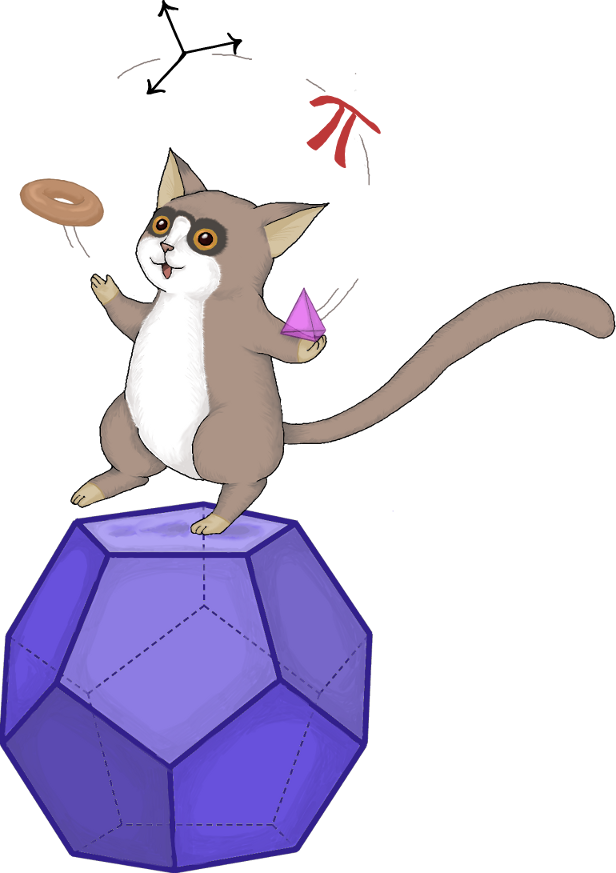
\includegraphics[scale=0.17]{cover}
  }
\end{picture} 

\vspace{6em}


\section*{Fraktale Dimensionen - Lösungshinweise}

Dieses Skript enthält Lösungs\emph{hinweise} zum letzten Korrespondenzbrief. Manchmal sind dies schon die kompletten Lösungen der Aufgaben, meistens sind es aber nur einige Hinweise, die dir dabei helfen sollen, auch die Aufgaben lösen zu können, bei denen du bisher nicht weiter gekommen bist. Wenn du noch weitere Fragen zu den Aufgaben hast, kannst du uns diese weiterhin gerne per E-Mail stellen.

Wenn du uns bereits deine eigenen Lösungsversuche geschickt hast (oder noch schicken wirst - das ist selbstverständlich immer noch möglich), dann versuchen wir natürlich auch dir mit unseren Korrekturen beim Verständnis der Aufgaben helfen. Es lohnt sich also uns deine Lösungen zu senden :-)

\begin{aufgabe}{}
	Mit der gleichen Überlegung wie für den zweiten Schritt erhält man:
	\begin{itemize}
		\item Nach $3$ Schritten eine Länge von $\left(\frac{4}{3}\right)^3\cdot l = \frac{4}{3}\cdot\frac{4}{3}\cdot\frac{4}{3}\cdot l = \frac{64}{27}l \approx 2,37 \cdot l$
		\item Nach $5$ Schritten eine Länge von $\left(\frac{4}{3}\right)^5\cdot l = \frac{4}{3}\cdot\frac{4}{3}\cdot\frac{4}{3}\cdot\frac{4}{3}\cdot\frac{4}{3}\cdot l  \approx 4,21 \cdot l$
		\item Nach $n$ Schritten eine Länge von $\left(\frac{4}{3}\right)^n\cdot l$
	\end{itemize}
\end{aufgabe}

\begin{aufgabe}{Wo ist der Schnee?}
	\begin{wrapfigure}{r}{.4\textwidth}\vspace{-1cm}
		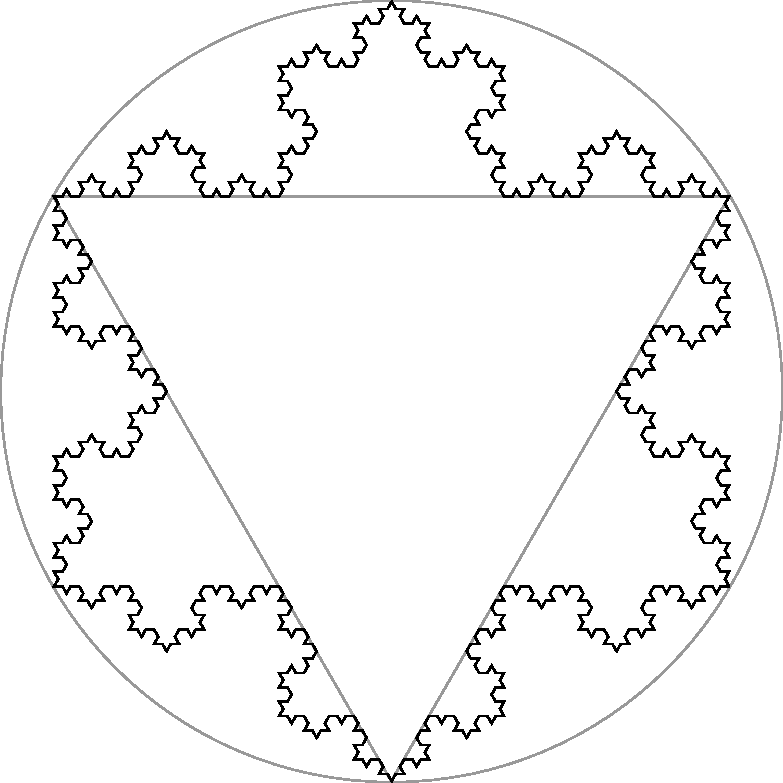
\includegraphics[width=.4\textwidth]{Bilder/Schneeflocke-Umkreis.pdf}
	\end{wrapfigure}

Der Umfang der Kochschen Schneeflocke ist offenbar dreimal so lang wie die Länge einer der drei Kochschen Kurven, aus denen sie besteht. Da deren Länge aber schon unendlich ist, ist natürlich auch der Umfang der Kochschen Schneeflocke unendlich.

Interessanterweise ist aber der Flächeninhalt der Kochschen Schneeflocke trotzdem endlich. Zum Beispiel kann man sich leicht überlegen, dass der Flächeninhalt kleiner sein muss als der des Umkreises des ursprünglichen Dreiecks - und der ist sicher endlich.

% Wenn man den Flächeninhalt exakt bestimmen möchte...  \[1 + \frac{1}{3} + \left(\frac{1}{3}\right)^2 + \dots = ???\]
\end{aufgabe}

\newpage

\begin{aufgabe}{Wie oft?}\label{aufgabe:Wie_oft}
\begin{center}
	\renewcommand{\arraystretch}{2}
	\begin{tabular}{l||c|c|c|c}
		Streckfaktor:& $2$-fach & $3$-fach & $4$-fach & $9$-fach \\\hline\hline
		Strecke      & $2$-mal	& $3$-mal  & $4$-fach & $9$-fach \\\hline
		Dreieck      & $4$-mal  & $9$-mal  & $16$-fach & $81$-fach \\\hline
		Quadrat      & $4$-mal  & $9$-mal  & $16$-fach & $81$-fach  \\\hline
		Würfel       & $8$-mal  & $27$-mal  & $64$-fach & $729$-fach  \\\hline
		Kochschee Kurve & ---   & $4$-mal  & ---      & $16$-mal  \\      	
	\end{tabular}
\end{center}
\end{aufgabe}

\begin{aufgabe}{Potenzen und Dimensionen}
\begin{center}
	\renewcommand{\arraystretch}{2}
	\begin{tabular}{l||c|c|c|c}
				      & $2$ & $3$ & $4$ & $9$ \\\hline\hline
		$\boxed{\phantom{1}}^1$  & $2^1=2$	& $3^1=3$ & $4^1=4$  & $9^1=9$ \\\hline
		$\boxed{\phantom{1}}^2$  & $2^2=4$	& $3^2=9$ & $4^2=16$ & $9^2=81$\\\hline
		$\boxed{\phantom{1}}^3$  & $2^3=8$	& $3^3=27$ & $4^3=64$ & $9^3=729$ \\\hline
		$\boxed{\phantom{1}}^{1,262}$  & $2,398$ & $4,001$ & $5,752$ & $16,005$     	
	\end{tabular}
\end{center}

Es fällt auf (in den ersten drei Zeilen): Streckt man ein $d$-dimensionales Objekt um den Faktor $k$, so passt das ursprüngliche genau $k^d$ in das neue. Das passt also genau zu unserer Definition 2 aus dem Korrespondenzbrief.

Damit diese Regel auch für die Kochsche Kurve gilt, müssen wir diese anscheinend als (ungefähr) $1,262$-dimensionales Objekt bezeichnen.

\end{aufgabe}

\begin{aufgabe}{}
	\begin{minipage}[t]{0.5\textwidth}
			\renewcommand{\arraystretch}{2}
			\begin{tabular}{l||c|c}
				Streckfaktor:& $2$-fach & $4$-fach \\\hline\hline
				Fraktal-Baum & $3$-mal & $9$-mal \\	
			\end{tabular}
	\end{minipage}
 

		
	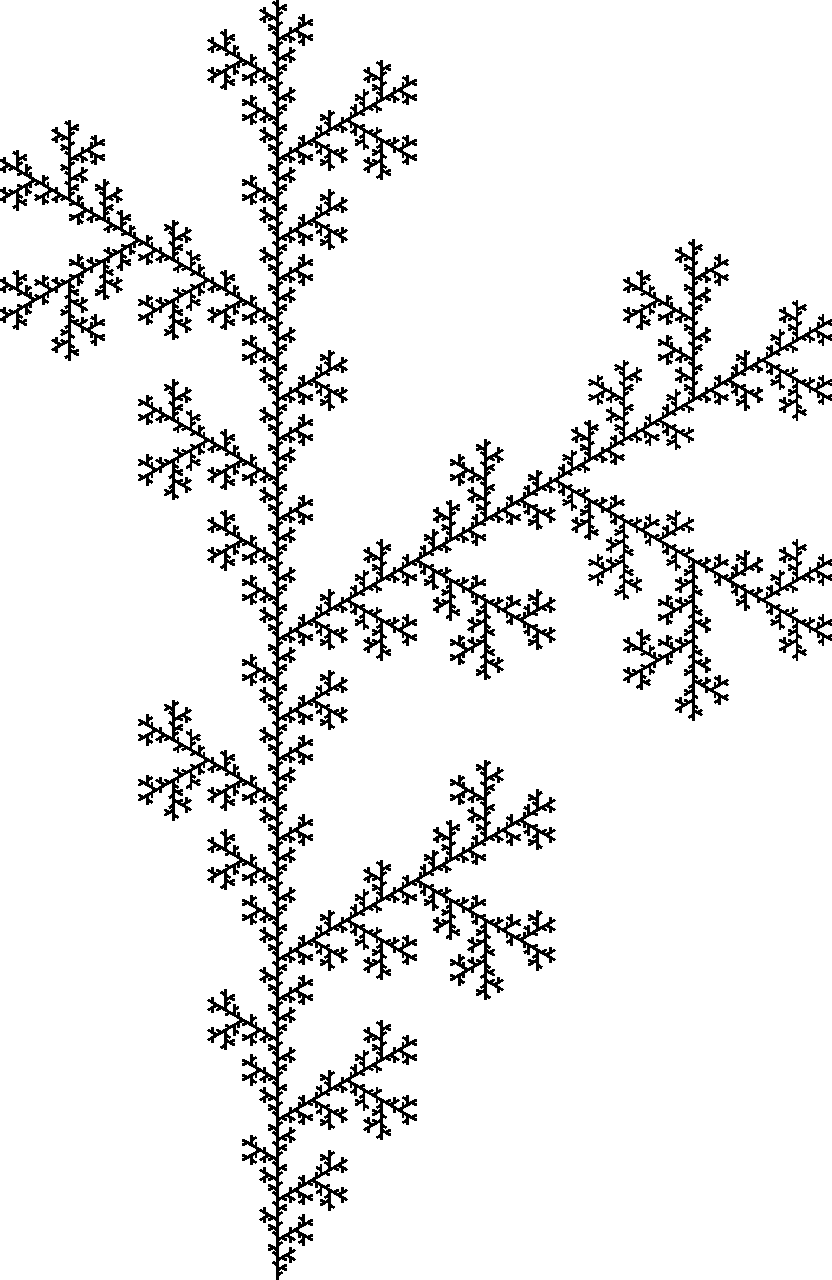
\includegraphics[width=.2\textwidth]{Bilder/Baum.pdf}
	$d \approx 1,585$
\end{aufgabe}

	\begin{minipage}[h]{5cm}
		Hello World
	\end{minipage}
	
	\begin{minipage}[h]{5cm}
		Hello World
	\end{minipage}

\subsection{Das Sierpinski-Dreieck}

\begin{center}
	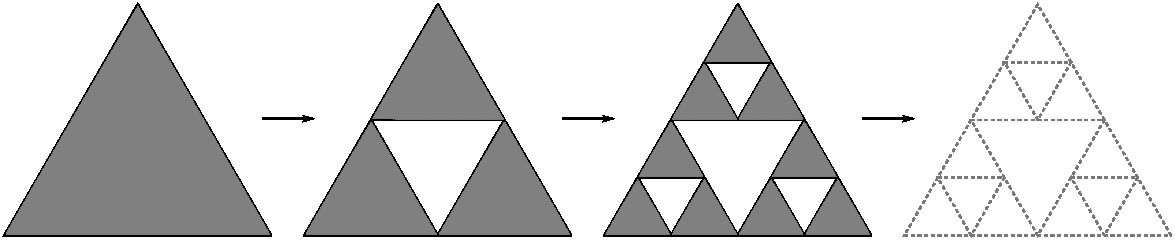
\includegraphics[width=.7\textwidth]{Bilder/Sierpinski-Konstruktion.pdf}
\end{center}

\begin{aufgabe}{}\label{aufgabe:Sierpinski-Flaeche}
	Strecken um 2 - passt 3-mal hinein. Also erneut $d \approx 1,585$
\end{aufgabe}

\begin{aufgabe}{}
	In jedem Schritt verliert man $\frac{1}{4}$ der grauen Fläche. Es bleiben also noch $\frac{3}{4}$. Nach $n$ Schritten also noch $\left(\frac{3}{4}\right)^n$. Der Flächeninhalt wird dadurch kleiner als jede positive Zahl. Folglich ist er $0$.
\end{aufgabe}

\begin{aufgabe}{Pascalsches Dreieck}
	TODO: Ausgefülltes und -gemaltes Pascalsches Dreieck.
	
	Man erhält das Muster des Sierpinski-Dreiecks.
\end{aufgabe}

\begin{aufgabe}{}
	Strecken um 3 -> passt 2-mal hinein. Also $d \approx 0,631$
	
	Nach jedem Schritt nur noch $\frac{2}{3}$ der Länge. Nach $n$ Schritten also noch $\left(\frac{2}{3}\right)^n$. Wird daher 0.
\end{aufgabe}

\begin{aufgabe}{}
	Strecken um 2 und passt 5-mal hinein. Also $d \approx 2,322$.
\end{aufgabe}
	
\begin{aufgabe}{}
	Fraktale Dimension größer als $2$. Daher Fläche (2-dimensional) unendlich. Kleiner als $3$, daher Volumen (3-dimensional) gleich 0.
	
	Fläche nach einem Schritt $\frac{5}{4}$-mal so groß und Volumen $\frac{5}{8}$-mal (5 Pyramiden, die jeweils halb so breit, halb so tief und halb so hoch sind.)
\end{aufgabe}

\begin{aufgabe}{}
	2-mal so groß, dann passt es 4-mal hinein. Damit ist $d = 2$. 
	
	Dieses Objekt ist flächenfüllend (d.h. wie eine Fläche - 2-dimensional)
\end{aufgabe}

\end{document}
